\section{Displaying the Mesh}
\label{section:DisplayingMeshes}

Upon successful creation of a mesh, you either need to load it in manually via the \ui{open MOAB file dialog} accessed from the \ui{open MOAB file item} in the \ui{file menu}, or, if you've just meshed an INP file you had loaded in previously, the mesh will load in automatically.


\subsection{Views of the Mesh}
To control viewing the mesh, be sure to click on the \ui{mesh tab} of the \ui{inputs panel}.  RGG allows you to six different options to control the \ui{Mesh view} of the mesh inside a drop down box (Figure \ref{fig:meshViews}), listed below:

\begin{wrapfigure}{R}{0.40\textwidth}
        \vspace{-4.5cm}
	\begin{center}
		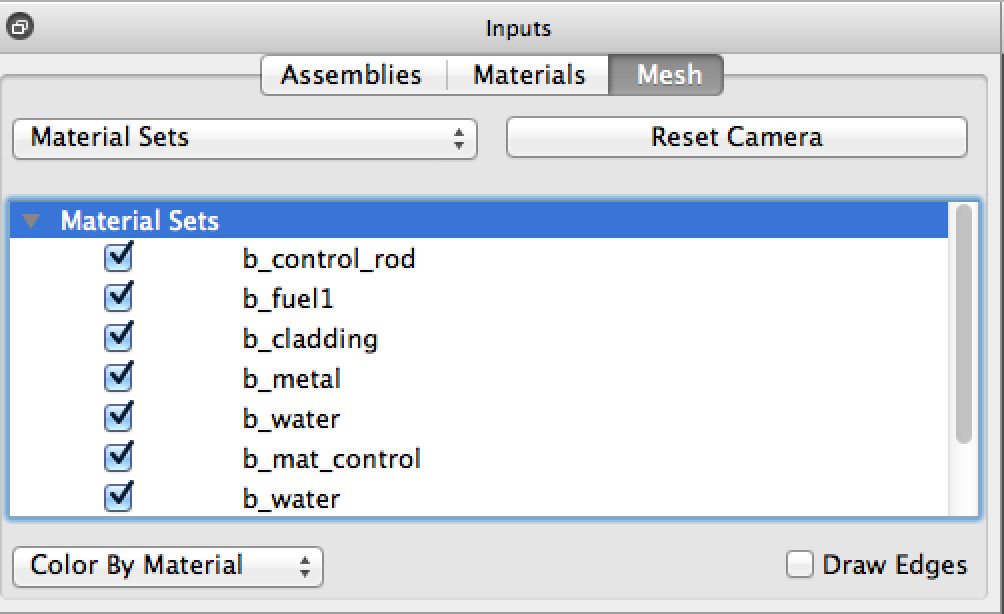
\includegraphics[width=0.95\linewidth]{Images/mash-tab.png}
		\caption{Used to control the mesh}
		\label{fig:mainwindow4}
	\end{center}
	\vspace{10pt}
	\begin{center}
		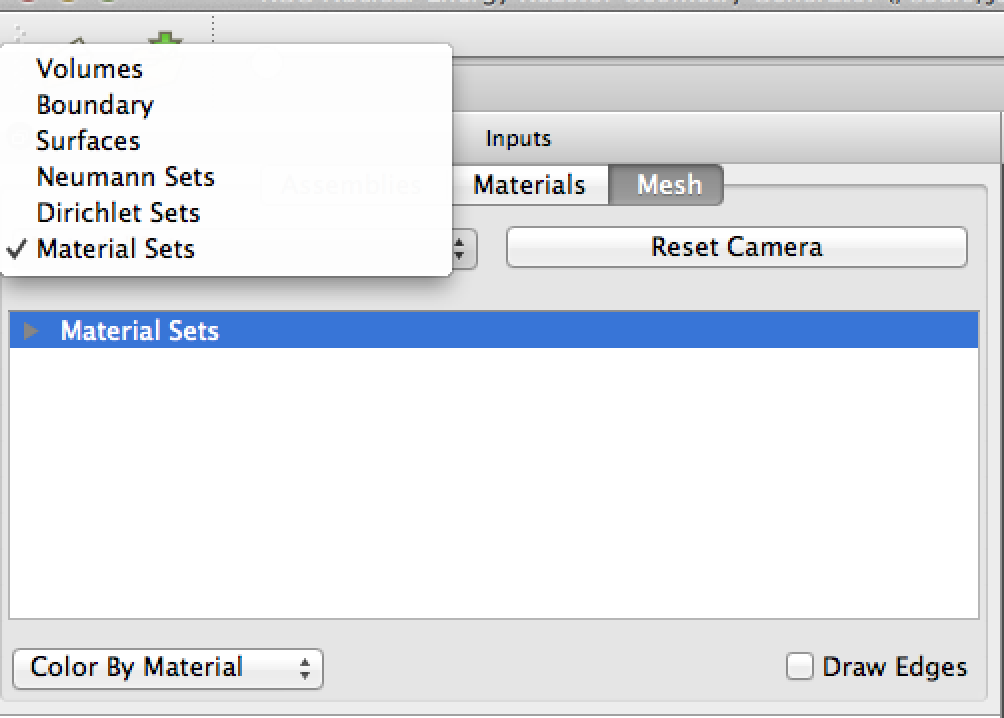
\includegraphics[width=0.95\linewidth]{Images/overview-of-mesh-options.png}
		\caption{The Views}
		\label{fig:meshViews}
	\end{center}
	\vspace{-1.5cm}
\end{wrapfigure}

\begin{itemize}
	\item{Volumes}
	\item{Boundary}
	\item{Surfaces}
	\item{Neumann Sets}
	\item{Dirichlet Sets}
	\item{Material Sets}
\end{itemize}


More detail on these views is provided below.  When available, we allow you to select a subsection for the selected option.  When selected, only that part is displayed int he Mesh View.  Also, using the checkboxes, one can hide a subsection (Figure \ref{fig:subsectionMesh}).  Additionally, you can check the \ui{show edges checkbox} to view the mesh superimposed on the Mesh View and check the \ui{color checkbox} to colorize the different pieces of the view based on the option you've selected.

\subsubsection{Volumes}
Clicking the \ui{volumes option} shows all the volumes of the mesh.  Checking the color checkbox will colorize all of the distinct volumes in different colors.

\subsubsection{Boundary}
When the \ui{Boundary option} is selected, RGG displays only the boundary conditions.  Checking the color checkbox will colorize all of the distinct volumes in different colors.

\subsubsection{Surfaces}
When the \ui{surfaces option} is selected, RGG displays only the surfaces of the mesh.

\begin{wrapfigure}{R}{0.45\textwidth}
	\begin{center}
		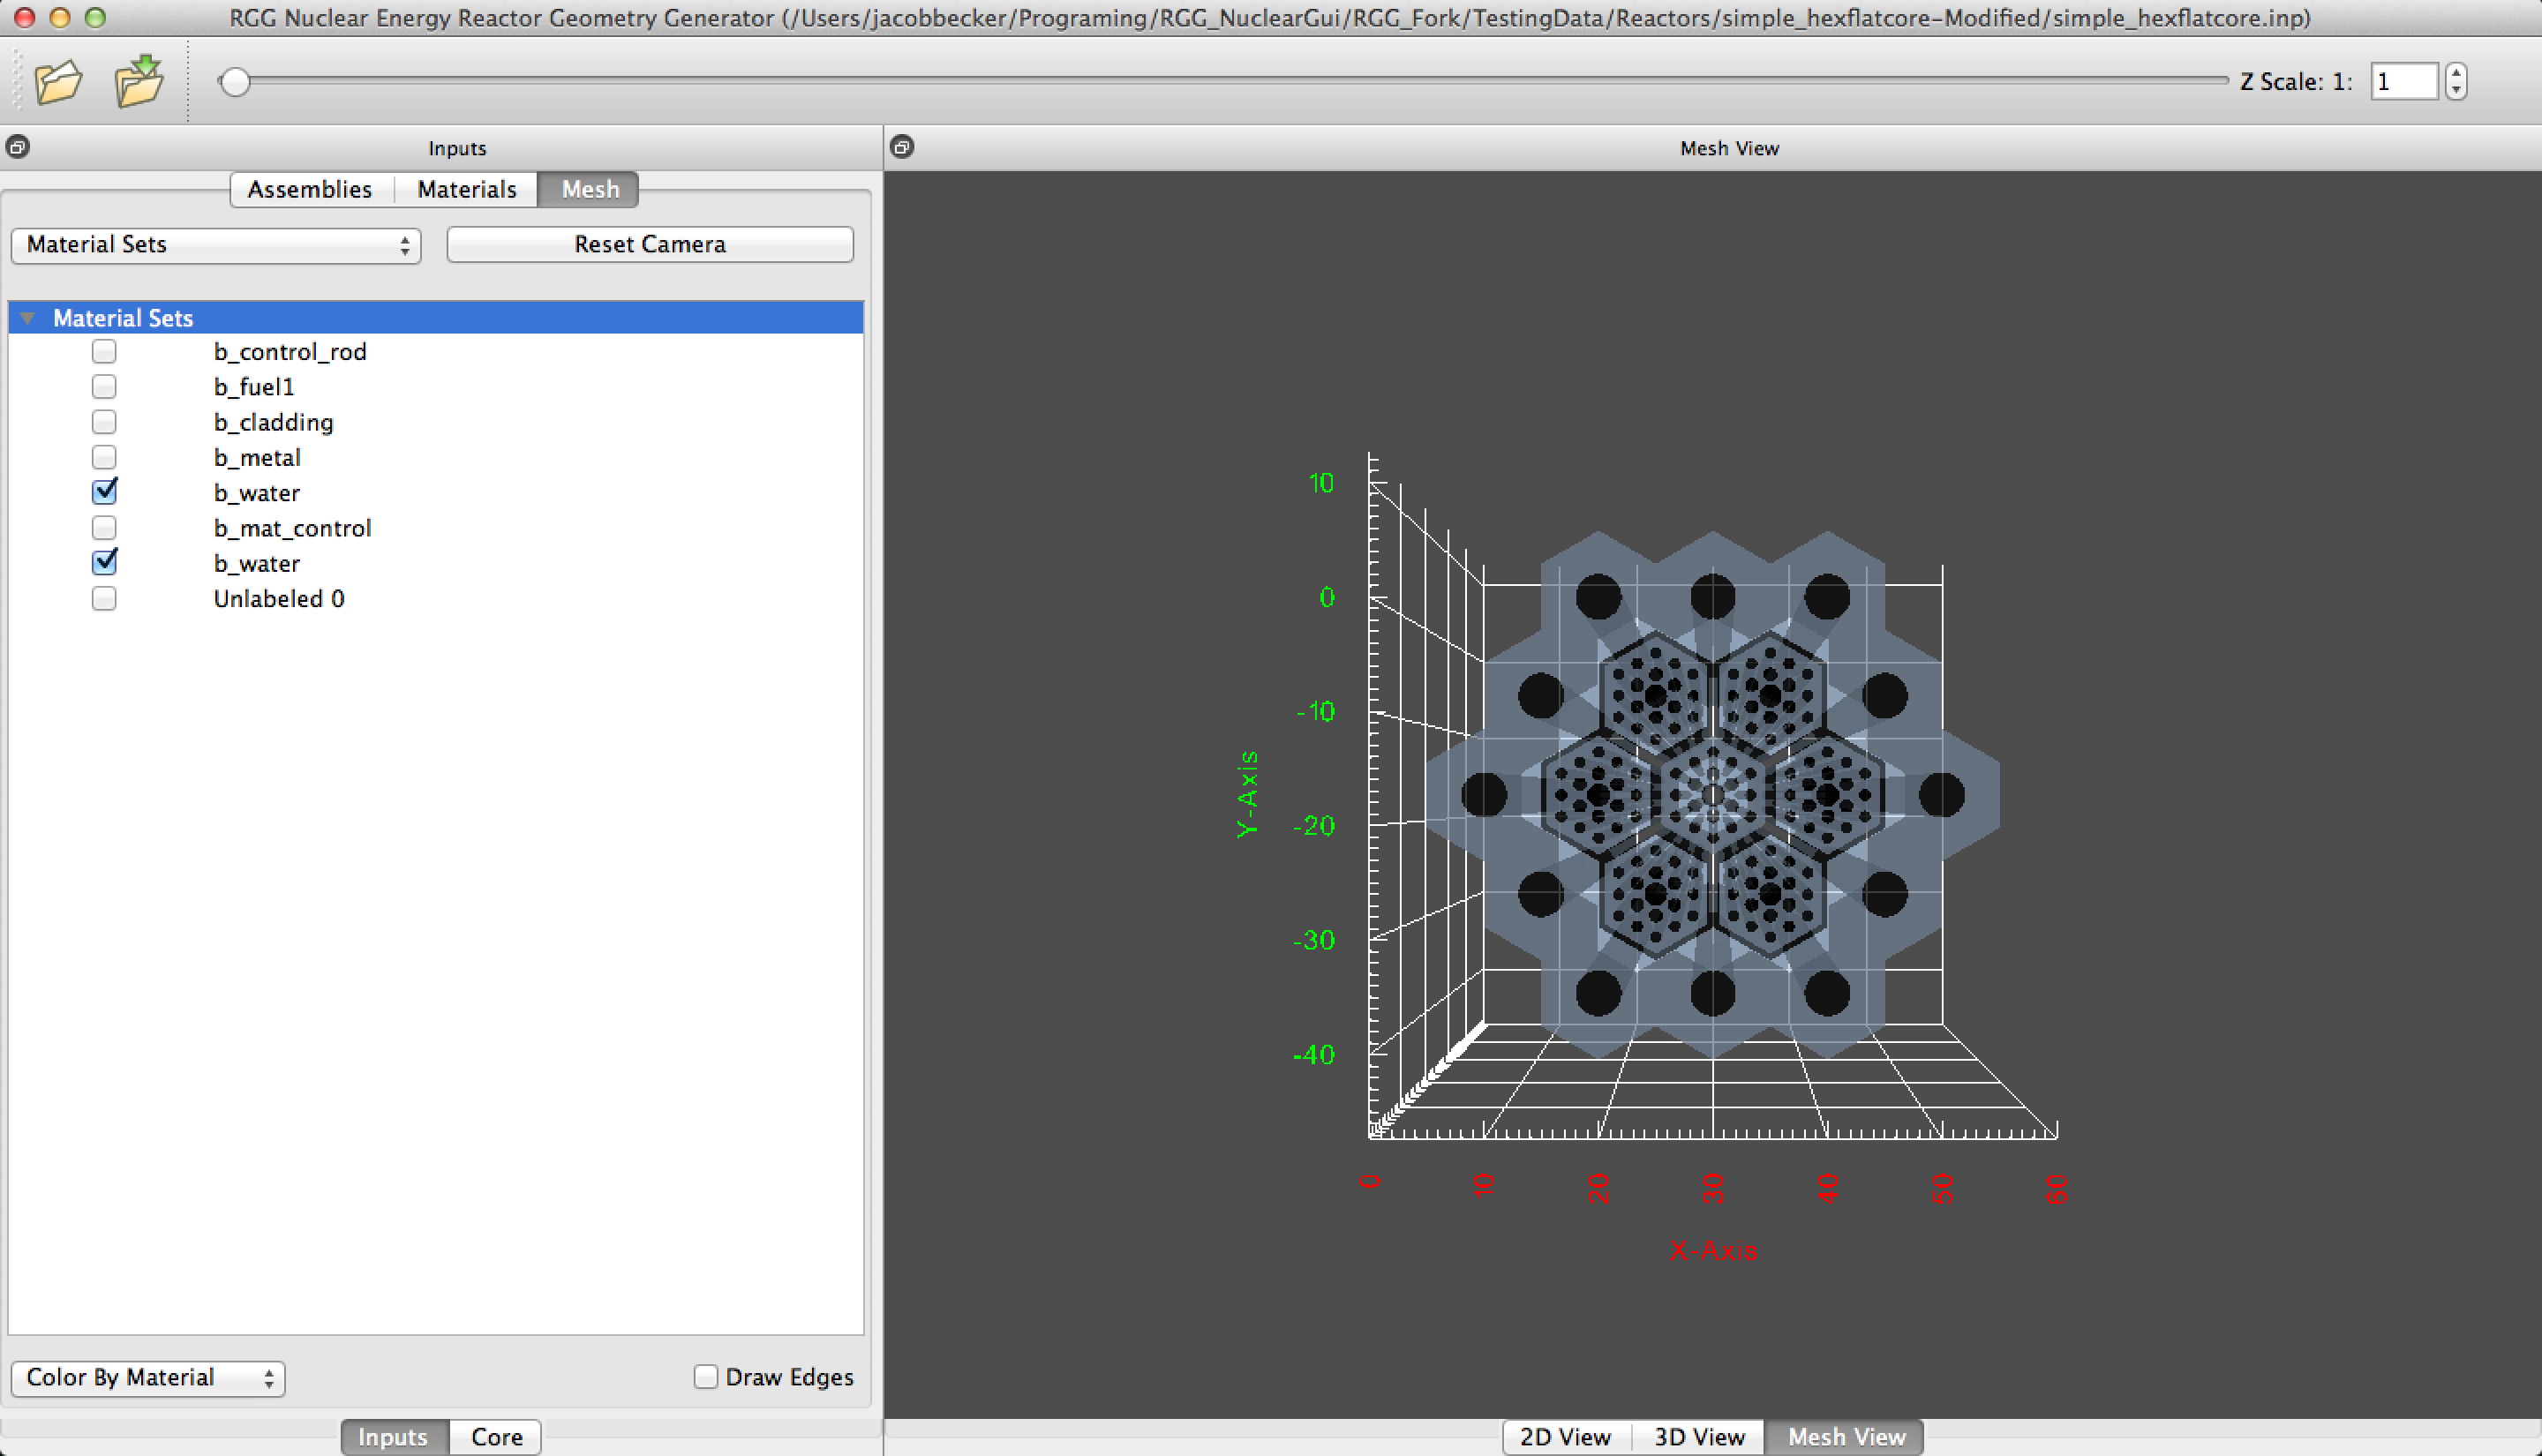
\includegraphics[width=0.95\linewidth]{Images/mesh-selection.png}
		\caption{All but water subsection are hidden}
		\label{fig:subsectionMesh}
	\end{center}
	\vspace{-5.cm}
\end{wrapfigure}

\subsubsection{Neumann Sets}
Clicking the \ui{Neumann Sets option} will show the natural boundary conditions on sides of domains.

\subsubsection{Dirichlet Sets}
Clicking the \ui{Dirichlet Sets option} will show the essential boundary conditions on points of domains.

\subsubsection{Material Sets}
The \ui{material sets} option displays all the volumes of the mesh, but colorizes them on a per material basis.  Additionally, you can toggle the visability of materials by checking and unchecking them in the \ui{materials tab} of the inputs panel.